\apendice{Documentación técnica de programación}

\section{Introducción}

En este apéndice se detallan aspectos relacionados a la documentación técnica. Se describirá la estructura de directorios, un apartado dedicado al montaje de desarrollo con el cual se ha trabajo, y un último apartado, dedicado a pruebas del sistema.

\section{Estructura de directorios}

La estructura de directorios (ver figura \ref{fig:estructura_github}) del repositorio GitHub contienen la aplicación web, la API y la documentación del trabajo.

\begin{figure}[h!] 
\centering
    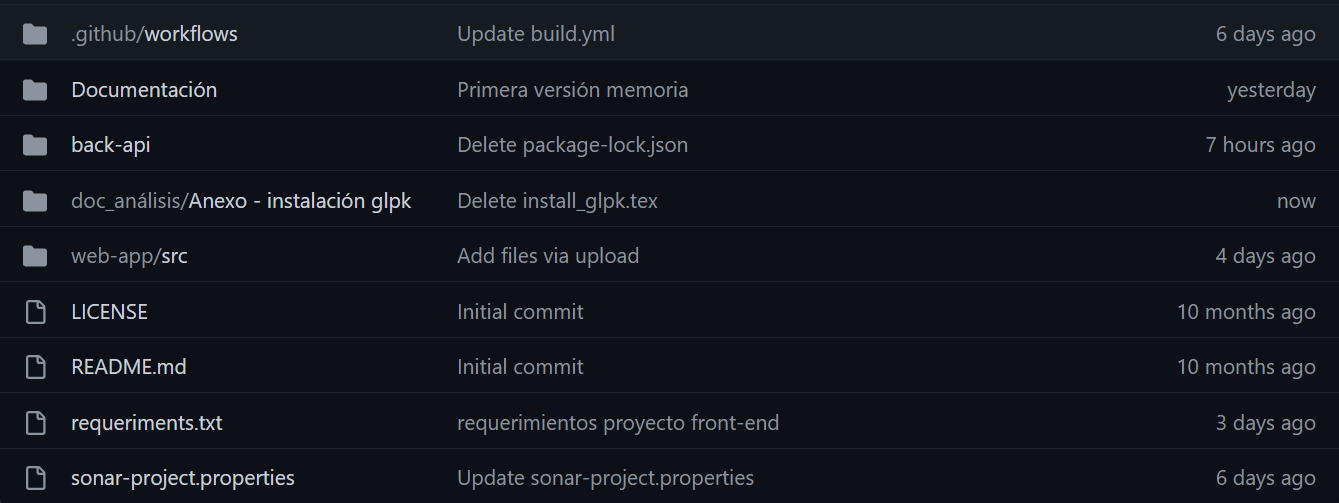
\includegraphics[width=0.8\textwidth]{img/estructura_github.PNG}
\caption{Estructura directorios, repositorio GitHub}
\label{fig:estructura_github}
\end{figure}

\subsection{.github.workflows}

Contiene archivos de configuración para el análisis de los códigos desde la herramienta Sonarcloud.

\subsection{Documentación}

Este directorio contiene los documentos de la memoria y los anexos. Así como los archivos .tex y las imágenes que forman los documentos.

\subsection{back-api}

Carpeta contiene el código de la API, que es un proyecto Laravel. Es importante destacar que este documento \textbf{no se ha usado en la parte de la subida al servidor}. Debido a problemas con la instalación de la librería GLPK \cite{glpk:package}. Pero hemos querido añadirlo, ya que ha sido un proyecto que ha servido como aprendizaje sobre como se comunican un proyecto front con un back.


\subsection{doc\_análisis}

Carpeta contiene documentos de análisis en \LaTeX. Algunas partes de estos documentos se han añadido a la memoria. Pero en su mayoría su objetivo ha sido documentar algunas lecturas interesantes del proceso de aprendizaje de herramientas. Y realizar algún documento de práctica con la nomenclatura de \LaTeX.


\subsection{web-app}

En este directorio hemos subido el contenido de la carpeta \textbf{src} del proyecto Angular. En la figura \ref{fig:src_angular} podemos ver los directorios default que tiene cualquier proyecto de angular.

\begin{figure}[h!] 
\centering
    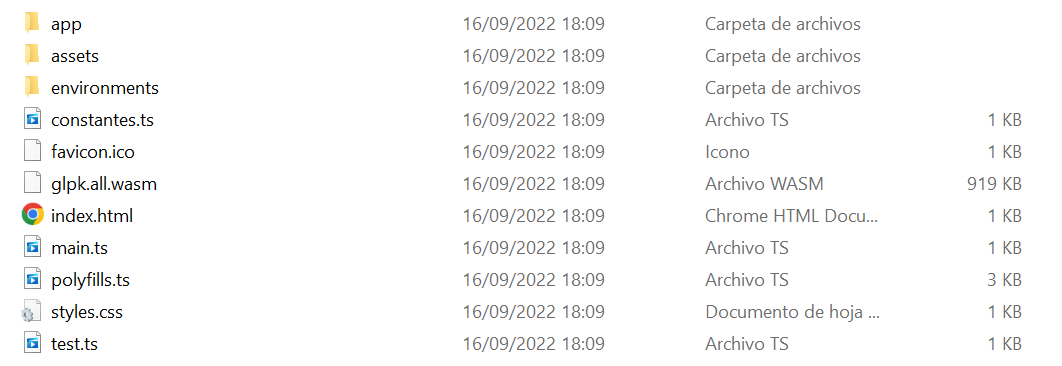
\includegraphics[width=0.8\textwidth]{img/src_angular.PNG}
\caption{Estructura directorio web-app/src}
\label{fig:src_angular}
\end{figure}

\begin{itemize}
    \item \textbf{Directorio app:} index.html es la página que contiene los componentes de las aplicaciones Angular. Estos componentes se encuentran dentro del directorio app (ver figura \ref{fig:app_angular}).
    
    \begin{figure}[h!] 
    \centering
        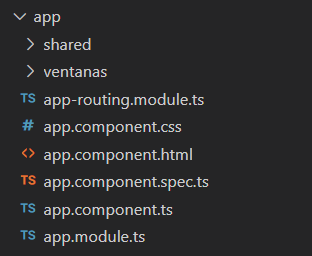
\includegraphics[width=0.8\textwidth]{img/app_angular.PNG}
    \caption{Estructura directorio web-app/src/app}
    \label{fig:app_angular}
    \end{figure}
    
    \newpage
    Directorios incluidos:
    
        \begin{itemize}
            \item \textbf{app-routing.module.ts:} contiene las rutas de la aplicación, están asignadas a componentes o módulos
            \item \textbf{app.component.css:} hoja de estilos del archivo \textit{app.component.html}
            \item \textbf{app.component.html:} archivo con la vista de la aplicación, archivo al que se apunta desde \textit{index.html}.
            \item \textbf{app.component.spec.ts:} archivo de pruebas del componente \textit{AppComponent}, que es el componente inicial de la aplicación.
            \item \textbf{app.component.ts:} archivo incluye la lógica del componente de arranque.
            \item \textbf{app.module.ts: }contiene la configuración de los imports y exports de módulos y componentes.
            \item \textbf{carpeta shared: } se ha configurado como un módulo que contiene componentes comunes en toda la aplicación.
            \item \textbf{carpeta ventanas:} contiene los componentes de las rutas principales de la aplicación.
        \end{itemize}
    
    \item \textbf{Directorio assets:} es el encargado de almacenar elementos estáticos como imágenes, pdfs, archivos mp3, etc (ver figura \ref{fig:assets_angular}).
    
    \begin{figure}[h!] 
    \centering
        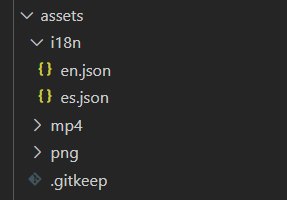
\includegraphics[width=0.8\textwidth]{img/assets_angular.PNG}
    \caption{Estructura directorio web-app/src/assets}
    \label{fig:assets_angular}
    \end{figure}
    
    \newpage
    Directorios incluidos:
    
    \begin{itemize}
        \item \textbf{Carpeta i18n:} contiene los archivos \textit{.json} con las traducciones tanto al inglés como al español.
        \item \textbf{Carpeta mp4:} contiene archivos con formato \textit{.mp4}, en este caso únicamente el vídeo guía de uso de la aplicación.
        \item \textbf{Carpeta png:} carpeta que contiene todas las imágenes e iconos usados en la aplicación
    \end{itemize}
    
    
    \item \textbf{Directorio environments:} nos permitir definir configuraciones para desplegar en un entorno local o producción.
    \item \textbf{constantes.ts:} archivo destinado a definir constantes globales para toda la aplicación.
    \item \textbf{favicon.ico:} es $16x16$ icon que sirve de icono de la web, permitiendo localizar al usuario la aplicación cuando se trabaja con múltiples ventanas
    \item \textbf{glpk.all.wasm:} archivo librería instalada GLPK.
    \item \textbf{index.html:} estructura inicial de documento HTML5; en este archivo se realiza la carga de scripts, estilos y dependencias necesarias. Además este archivo hace una llamada al fichero \textit{favicon.ico}
    \item \textbf{main.ts:} Este fichero es el encargado de definir qué módulo es el de arranque. Apuntando normalmente al AppComponent.
    \item \textbf{polyfills.ts:} Contiene algunos archivos para que nuestra aplicación sea compatible con algunos navegadores antiguos. El código se transpila a ES6 que no es compatible con algunas versiones de Internet Explorer o Firefox (ES5 si que es compatible) 
    \item \textbf{styles.css:} hoja de estilos asociada al archivo \textit{index.html}. Es llamado desde el archivo \textit{angular.json} configurándolo como la hoja principal de estilos de la aplicación.
    \item \textbf{test.ts:} Define la configuración que va a utilizar Karma. En este archivo se define el entorno de prueba.
\end{itemize}

\subsection{Ficheros adicionales}

\begin{itemize}
    \item \textbf{LICENSE:} archivo contiene información referente a la licencia marcada en el repositorio.
    \item \textbf{README.md:} Archivo presentación del repositorio GitHub y del proyecto.
    \item \textbf{requeriments.txt:} contiene parte del archivo \textbf{package.json} del proyecto en Angular. Está formado por las dependencias de la aplicación, y se usa en el proceso de montaje del proyecto. 
    \item \textbf{sonar-project.properties:} archivo de configuración de SonarCloud en el repositorio
\end{itemize}

\section{Manual del programador}

En esta sección se va a realizar la configuración de un entorno de desarrollo con las herramientas principales con las que se ha trabajado.

\subsubsection{Instalación Visual Studio Code}

Visual Studio Code se ha usado como framework de desarrollo. Se puede descargar mediante en enlace \url{https://code.visualstudio.com/download}, donde podremos descargar la versión correspondiente a nuestro sistema operativo.

Algunas de las extensiones que hemos utilizado en el desarrollo son (figura \ref{fig:visualstudio_extensions}):

\begin{figure}[h!] 
\centering
    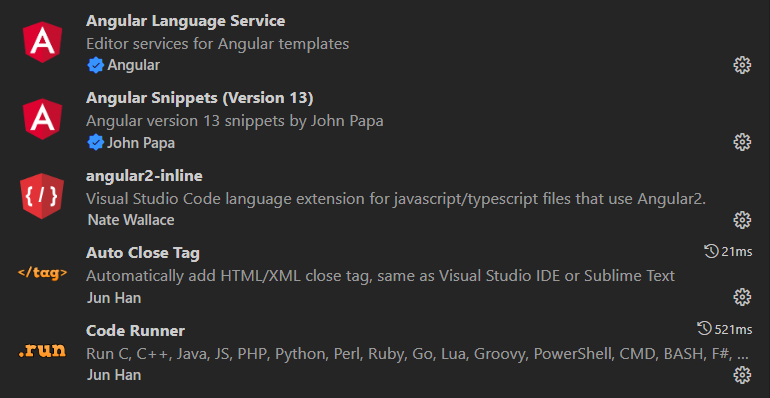
\includegraphics[width=1\textwidth]{img/visualcode_extensiones.PNG}
\caption{Visual Studio Code extensiones}
\label{fig:visualstudio_extensions}
\end{figure}

\subsubsection{Instalación Postman}

Para ejecutar las pruebas funcionales de la API, hemos utilizado la herramienta Postman que se puede descargar en el siguiente link de descarga: \url{https://www.postman.com/downloads/}

\subsubsection{Instalación Nodejs y npm}

Para el proyecto angular es necesario tener una versión de Nodejs instalada. Podemos obtener este link de descarga en su página oficial: \url{https://nodejs.org/es/download/}, seleccionando la versión dependiendo nuestro sistema. Después de la instalación es recomendable reiniciar el equipo.

\subsubsection{Instalación Debian}

Hemos usado Debian para simular un subsistema Linux en un sistema principal Windows. Link de descarga en: \url{https://apps.microsoft.com/store/detail/debian/9MSVKQC78PK6?hl=es-es&gl=es}


\section{Compilación, instalación y ejecución del proyecto}

Para utilizar el proyecto es necesario dirigirse al Github en \url{https://github.com/humbertoms99/Mixing_models}, y descargar el zip del repositorio.

\subsection{Instalación Angular y librerías Node}

Previamente debemos tener instalado Nodejs, ya que vamos a necesitar ejecutar algunos comandos npm.

Nos posicionamos en la ruta donde queremos montar el proyecto y ejecutamos el comando \textit{npm install -g @angular/cli} que instalará las dependencias angular/cli.
Creamos un proyecto angular \textit{ng new mixing\_models} (ver figura \ref{fig:ng_new}), y entramos en la carpeta creada con \textit{cd mixing\_models}. El siguiente paso es instalar las librerías (Recomendable hacerlo con la opción más abajo): \\


\begin{figure}[h!] 
\centering
    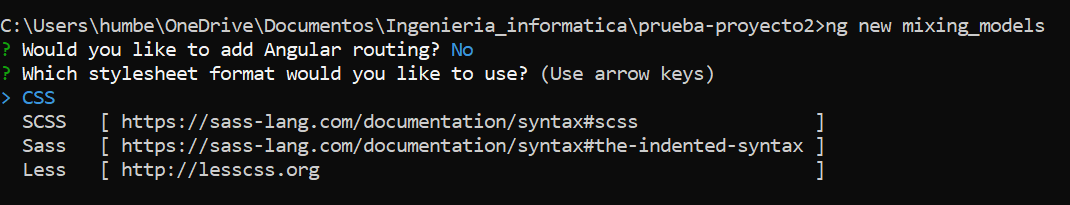
\includegraphics[width=0.8\textwidth]{img/ng_new.PNG}
\caption{Comando ng new nombre-proyecto}
\label{fig:ng_new}
\end{figure}

Instalación librería Fast Combinatorial Non-negative Least Squares:
$$ npm\:i\:ml-fcnnls $$
Instalación GLPK interface for TypeScript:
$$ npm\:install\:glpk-ts $$
Angular Material:
$$ ng\:add\:@angular/material  $$
Angular ngx-translate:
$$ npm\:install\:@ngx-translate/core\:@ngx-translate/http-loader $$
GLPK compiled to wasm:
$$ npm\:i\:glpk-wasm $$
Y los comandos:
$$ npm\:install\:@types/node\:--save-dev $$
$$ npm\:install\:@angular/localize\:--save $$

En vez de realizar estas instalaciones podemos abrir el archivo \textbf{package.json} y copiar el contenido de la carpeta \textit{requeriment.txt} del GitHub. Y copiar de esta forma las dependencias del proyecto, y para instalarlas ejecutamos el comando:

$$ npm\:install\:--legacy-peer-deps $$

En el archivo \textbf{angular.json}: 

\begin{figure}[h!] 
\centering
    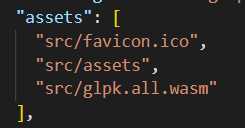
\includegraphics[width=0.8\textwidth]{img/angular_json.PNG}
\caption{Configuración angular - angular.json}
\label{fig:angular_json}
\end{figure}

En el archivo \textbf{tsconfig.json}: 

\begin{figure}[h!] 
\centering
    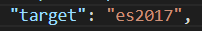
\includegraphics[width=0.8\textwidth]{img/tsconfig_json.PNG}
\caption{Configuración angular - tsconfig.json}
\label{fig:tsconfig_json}
\end{figure}

\newpage
El el archivo \textbf{tsconfig.app.json}

\begin{figure}[h!] 
\centering
    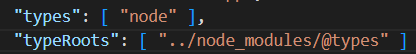
\includegraphics[width=0.8\textwidth]{img/tsconfig_app_json.PNG}
\caption{Configuración angular - tsconfig.app.json}
\label{fig:tsconfig_app_json}
\end{figure}

Por último, \textbf{borramos la carpeta src} y pegamos la carpeta src  que se encuentra dentro la carpeta web-app del zip descargado del repositorio del GitHub.

\subsection{Ejecución del proyecto}

Una vez configurado el proyecto, abrimos la terminal y nos posiciones en path del carpeta del proyecto con el comando:



Y para ejecutar la aplicación:

$$ ng\:serve\:-o $$

Con este comando no abrirá automáticamente una ventana en nuestro navegador, con la dirección \textit{http://localhost:4200/} 



\section{Pruebas del sistema}

Las pruebas de sistema validan el sistema completo y totalmente integrado. El objetivo de las pruebas de sistema es evaluar las especificaciones del sistema en su totalidad.

Para realizar estas pruebas hemos utilizado la herramienta SonarCloud que es una plataforma para evaluar la calidad del código fuentes. Es una herramienta de software libre y está vinculada con GitHub para obtener métricas de calidad de código.

Para poder realizar los análisis se han añadido los archivos \textit{sonar-project.properties} y \textit{.github/workflows/build.yml} y una key en el apartado de configuración del respositorio de GitHub. Esto hace que Sonarcloud analicé el contenido actual de la carpeta del proyecto Github.

Podemos ver el resumen del análisis del código en la figura \ref{fig:sonarcloud_res}. 

\begin{figure}[h!] 
\centering
    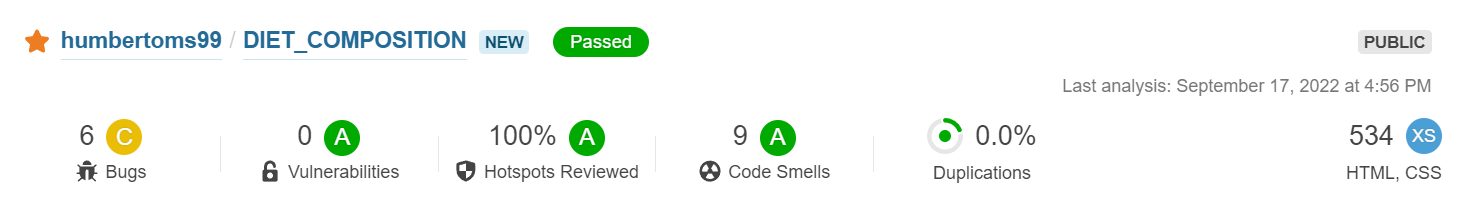
\includegraphics[width=1\textwidth]{img/sonarcloud_res_1.PNG}
\caption{Resumen análisis código Sonarcloud}
\label{fig:sonarcloud_res}
\end{figure}

\begin{itemize}
    \item \textbf{Bugs:} errores de código que pueden romper el código y deben ser corregidos cuando antes. 
    \item \textbf{Vulnerabilities:} partes del código que pueden ser explotadas por un hacker.
    \item \textbf{CodeSmells: } códigos que son confusos, y por tanto difíciles de mantener.
    \item \textbf{Security Hotspots: } código sensible a la seguridad que requiere una revisión manual para evaluar si existe o no una vulnerabilidad.
    \item \textbf{Duplications:} porcentaje de códigos duplicados en las nuevas líneas
    \item \textbf{Líneas de códigos y lenguajes utilizados.}
\end{itemize}

Además si accedemos a una rama concreta podemos ver análisis más específicos, como por ejemplo el listado de issues (figura \ref{fig:sonarcloud_issues}). Consideramos muy útil este apartado porque aparte de ofrecernos el listado completo de fallos pendientes por arreglar, nos da una aproximación de tiempo de cada issue y un tiempo total aproximado para todas, establece importancia y permite añadir etiquetas. Además permite asignar estas tareas al estar sincronizado con GitHub.

\begin{figure}[h!] 
\centering
    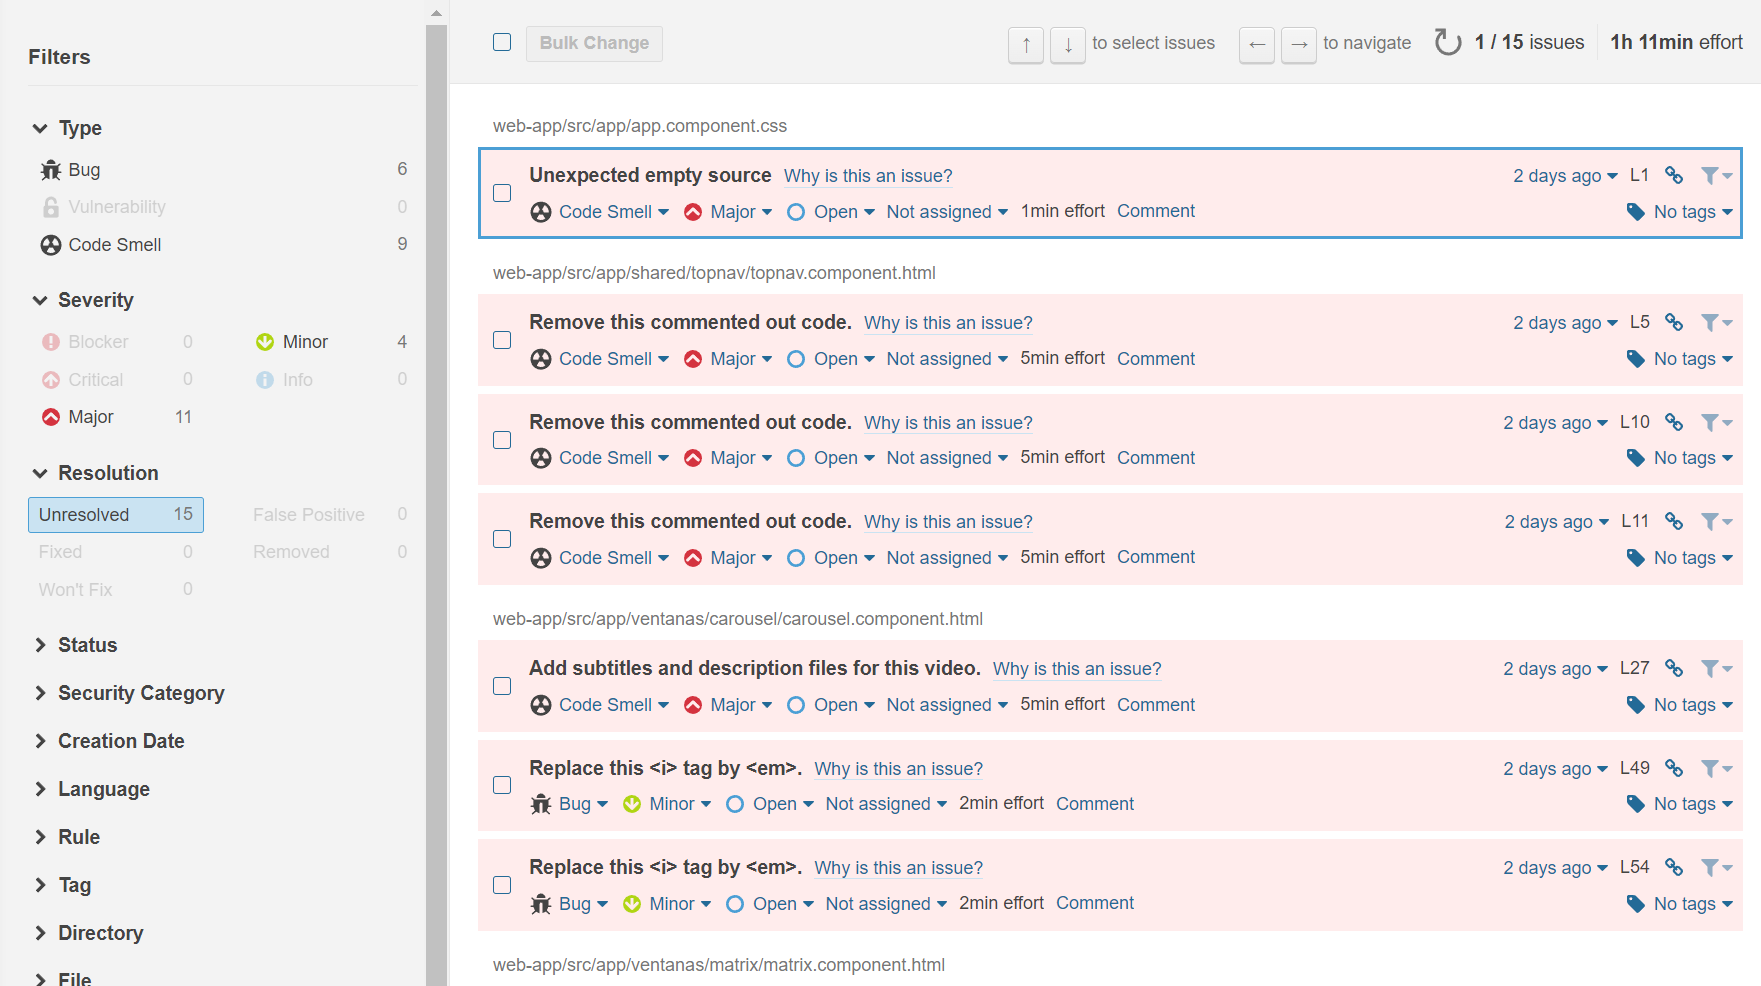
\includegraphics[width=1\textwidth]{img/sonarcloud_issues_1.PNG}
\caption{Sonarcloud issues brand main}
\label{fig:sonarcloud_issues}
\end{figure}

\newpage
Por último, podemos entrar al apartado de \textbf{Code} (ver figura \ref{fig:sonarcloud_lines_code}). En este apartado veremos un listado de todos los archivos, sus líneas de código y los Bugs, vulnerabilities, Code Smells, Security Hotspots, Coverage y Duplications. Apartado que puede servir para ver una visión general del código. 

\begin{figure}[h!] 
\centering
    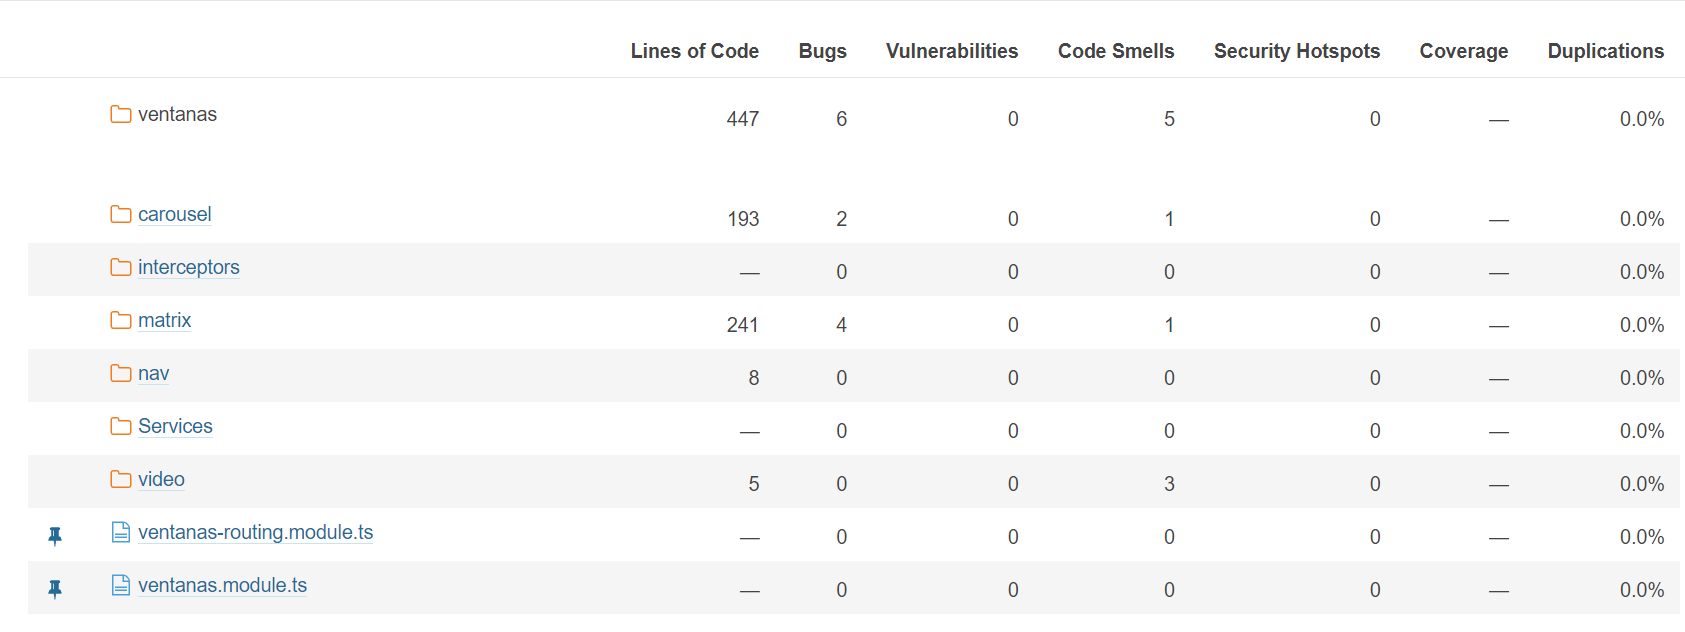
\includegraphics[width=1\textwidth]{img/sonarcloud_lines_code_1.PNG}
\caption{Sonarcloud líneas de código}
\label{fig:sonarcloud_lines_code}
\end{figure}


